\documentclass[12pt, a4paper]{article}
\usepackage{polyglossia}
\usepackage{geometry}
\usepackage{xcolor}
\usepackage{fontawesome5}
\usepackage{multicol}
\usepackage{enumitem} 
\usepackage{hyperref}
\usepackage[absolute]{textpos} 
\usepackage{graphicx}
\usepackage{fancybox}
\usepackage{tikz}

\setmainfont{CrimsonPro}
\newfontfamily\fonthead{AlegreyaSC}
\pagestyle{empty}
\setlength\parindent{0pt}

\setlength{\TPHorizModule}{1cm} % Horizontal unit = 1cm
\setlength{\TPVertModule}{1cm}  % Vertical unit = 1cm

\newcommand{\head}[1]{
  \section*{\fonthead{#1}}
}

\begin{document}

\newgeometry{top=1.2in}

\head{Murtahda Alkaibe}

\faEnvelope \, murtaza.alkibe@gmail.com \hspace{6pt}
\faGithub \, \underline{\href{https://github.com/Murtaza01}{Murtaza01}} \hspace{6pt} \smallbreak
\faPhone \, +964\,773\,9490\,391  \hspace{6pt} 
\faMap \, Iraq, Baghdad  \smallbreak
\faPaperPlane \, @Murtaza\_Alkaibe \hspace{6pt}
\faLinkedin \, \underline{\href{https://www.linkedin.com/in/murtaza-alkabie/}{murtaza-alkabie}}


\begin{textblock}{}(11.9,3) % (width is auto)
\begin{tikzpicture}
\node[rounded corners=24pt,  % Adjust radius (e.g., 8pt, 15pt)
        inner sep=0,           % No extra padding
        clip]                  % Clip image to rounded shape
  {
  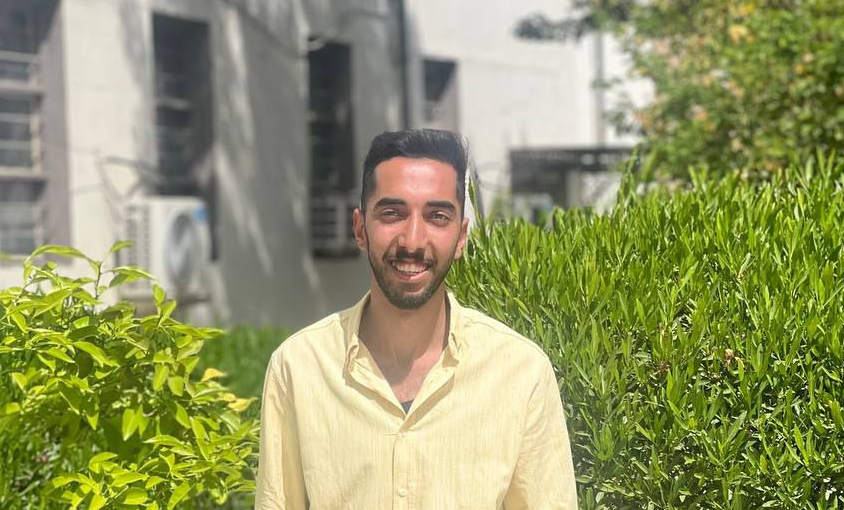
\includegraphics[width=6cm]{mertdha_pic.png}
};
  
\end{tikzpicture}

\end{textblock}
% Place image at (x=3cm, y=5cm) from top-left corner

\subsection*{Education}
\vspace{-0.4em}
\hrule\bigbreak

  \textbf{Bachelor in Computer Science}

   \textit{At College of Science, University of Baghdad}.\medbreak

  \textbf{Full Stack Bootcamp}

    \textit{At Re:Coded}.\medbreak

\textbf{English Training}

    \textit{At Ministry of Labour and Social Affairs}.
  

\subsection*{Experience}
\vspace{-0.4em}
\hrule\bigbreak

   \textbf{Freelancer as Web Developer}\medbreak

   \textbf{Literary Translator}

   \textit{At Beldash Publishing House}\smallbreak


\subsection*{Projects}
\vspace{-0.4em}
\hrule\bigbreak


\textbf{College Site | \underline{\href{https://english-section.netlify.app/}{GitHub}}}\smallbreak
Built and maintained a website for my college using \textbf{React router} for single page
application, \textbf{Redux} for saving logged users and 
\textbf{i18n} for internationalization.\bigbreak

\textbf{Survey Site | \underline{\href{https://sos-10-survey.netlify.app/}{GitHub}}}\smallbreak
Built and maintained a website for a survey with backend where i used \textbf{Nodejs} for
main backend code and \textbf{expressjs} as the framework, and \textbf{MySQL} for the 
database.\bigbreak

\textbf{Best Picture Site | \underline{\href{https://best-pic.netlify.app/}{GitHub}}}\smallbreak
Built and maintained a website that support uploading pictures through \textbf{cloudinary} and
competing with other people online. The site uses \textbf{MonogDB} for database.


\subsection*{Skills}
\vspace{-0.4em}
\hrule

\begin{multicols}{2} % 2 columns
    \begin{itemize}[noitemsep,topsep=0pt]
        \item Typescript \& Javascript.
        \item RestAPI \& GraphQL 
        \item MYSQL \& MangoDB.
        \item ReactJs \& AstroJs.
        \item NodeJs \& ExpressJs.
        \item Microsoft Office and LaTeX .
        \item CSS, Sass and Tailwind.
        \item English fluency \& Arabic Native.
        \item Arch Linux.
    \end{itemize}
\end{multicols}
  
\end{document}
